\chapter{Reaction Mechanisms: Elementary Steps and Approximations}\label{ch:b1:elementary-steps}

Nitrogen monoxide, formed in car engines and lightning, combines with the
oxygen of the air: \ce{2NO + O2 -> 2NO2}. Measured in the laboratory, the
rate of this reaction is proportional to $[\ce{NO}]^2[\ce{O2}]$ --- and it
goes \emph{slower} when the gas is heated. A single collision of three
molecules could explain the first fact, never the second: every
collision gets more energetic with temperature. The explanation is that
the reaction is not one event but a sequence of simpler ones, its
mechanism. This chapter defines these \omterm{def:b1:elementary-steps:elementary-step}{elementary steps}, the \omterm{def:b1:elementary-steps:energy-profile}{energy
profile} along which they run, and the approximations that turn a
mechanism into a \omterm{def:b1:rate-laws:order}{rate law}; it ends with catalysis, the art of opening an
easier path.

\begin{recall}
Book 1 (grade 12) described a \omterm{def:b1:elementary-steps:elementary-step}{reaction mechanism} as a sequence of steps
drawn with curly arrows, with intermediates formed and consumed, and a
\omterm{def:b1:elementary-steps:catalyst}{catalyst} as a species that speeds a reaction without being consumed.
\omterm{def:b1:rate-laws:order}{Rate laws}, orders and the \omterm{thm:b1:rate-laws:arrhenius}{Arrhenius law} were defined in
\cref{ch:b1:rate-laws}.
\end{recall}

\section{Elementary steps}

\begin{definition}[Elementary step, molecularity, mechanism]\label{def:b1:elementary-steps:elementary-step}
An \emph{elementary step}\index{elementary step} is a reaction that takes
place in a single molecular event, as it is written, without any
intermediate. Its \emph{molecularity}\index{molecularity} is the number of
particles that react in that event: 1 (unimolecular, a decomposition or
rearrangement), 2 (bimolecular, a collision), rarely 3. A \emph{reaction
mechanism}\index{reaction mechanism} is the set of elementary steps whose
sum is the overall reaction. A species formed in one step and consumed in
a later one, absent from the overall equation, is a \emph{reaction
intermediate}\index{reaction intermediate}.
\end{definition}

\begin{proposition}[Rate law of an elementary step]\label{prop:b1:elementary-steps:elementary-law}
An \omterm{def:b1:elementary-steps:elementary-step}{elementary step} has an order, and its \omterm{def:b1:rate-laws:order}{partial orders} equal its
stoichiometric coefficients: $\mathrm{A} \to \dots$ has $v = k[\mathrm{A}]$;
$\mathrm{A} + \mathrm{B} \to \dots$ has $v = k[\mathrm{A}][\mathrm{B}]$;
$2\,\mathrm{A} \to \dots$ has $v = k[\mathrm{A}]^2$. The converse is false:
a reaction whose orders equal its coefficients need not be elementary.
\end{proposition}

\begin{proof}[Reasoning]
A bimolecular step happens when an \ce{A} meets a \ce{B}; the number of
such encounters per unit volume and time is proportional to the number
of \ce{A} per unit volume and to the number of \ce{B}, hence to
$[\ce{A}][\ce{B}]$. A unimolecular step happens to each molecule with a
fixed probability per unit time, hence a rate proportional to $[\ce{A}]$.
\end{proof}

\begin{remark}[Why molecularity rarely exceeds two]\label{rem:b1:elementary-steps:termolecular}
Three particles meeting at the same instant, each with the right energy
and orientation, is a rare event; a reaction of \omterm{def:b1:rate-laws:order}{overall order} 3 is almost
always the result of two successive bimolecular steps, as in the
weekend problem.
\end{remark}

\section{Energy profiles}

\begin{definition}[Reaction coordinate, energy profile, transition state]\label{def:b1:elementary-steps:energy-profile}
Along an \omterm{def:b1:elementary-steps:elementary-step}{elementary step} the atoms move from the arrangement of the
reactants to that of the products; a variable that measures this progress
(a bond length that grows, another that shrinks) is the \emph{reaction
coordinate}\index{reaction coordinate}. The graph of the potential energy
of the system along it is the \emph{energy profile}\index{energy profile}.
Its maximum is the \emph{transition state}\index{transition state},
an arrangement of the atoms with bonds half-made and
half-broken, which lasts no longer than a molecular vibration and cannot
be isolated. The height of this maximum above the reactants is the
energy barrier of the step.
\end{definition}

\begin{omfigure}
\begin{tikzpicture}
\begin{axis}[omprofile, name=a,
  width=0.48\linewidth, height=5.4cm, xmin=0, xmax=10, ymin=-68, ymax=95,
  xlabel={reaction coordinate}, ylabel={energy}]
\addplot[omDef, very thick] table[x=x, y=E] {figdata/out/bachelor-1-energy-profiles-one-step.dat};
\draw[dashed, black!40] (axis cs:0,0) -- (axis cs:10,0);
\draw[<->, omThm] (axis cs:5,0) -- (axis cs:5,79);
\node[omThm, anchor=west, font=\small] at (axis cs:5.1,30) {barrier};
\draw[<->, omProp] (axis cs:9.9,0) -- (axis cs:9.9,-40);
\node[omProp, anchor=east, font=\small] at (axis cs:9.8,-14) {$\Delta E$};
\node[anchor=south, font=\small] at (axis cs:5,81) {transition state};
\node[anchor=north west, font=\small] at (axis cs:0.15,-3) {reactants};
\node[anchor=north, font=\small] at (axis cs:8.6,-42) {products};
\end{axis}
\begin{axis}[omprofile, at={(a.east)}, anchor=west, xshift=1.2cm,
  width=0.48\linewidth, height=5.4cm, xmin=0, xmax=10, ymin=-64, ymax=95,
  xlabel={reaction coordinate}, ylabel={energy}]
\addplot[omDef, very thick] table[x=x, y=E] {figdata/out/bachelor-1-energy-profiles-two-step.dat};
\node[anchor=south, font=\small] at (axis cs:3,71) {TS 1};
\node[anchor=south, font=\small] at (axis cs:7,56) {TS 2};
\node[anchor=north, font=\small, align=center] at (axis cs:5,27) {inter-\\mediate};
\node[anchor=north west, font=\small] at (axis cs:0.15,-3) {reactants};
\node[anchor=north east, font=\small] at (axis cs:10,-43) {products};
\end{axis}
\end{tikzpicture}

{\small Left: the profile of one \omterm{def:b1:elementary-steps:elementary-step}{elementary step}, with its barrier and the
energy change of the reaction. Right: a two-step mechanism; the
intermediate sits in a hollow between two \omterm{def:b1:elementary-steps:energy-profile}{transition states}. The
energies are illustrative.}
\end{omfigure}

\begin{proposition}[Barriers and the Arrhenius law]\label{prop:b1:elementary-steps:barrier}
The \omterm{def:b1:rate-laws:activation-energy}{activation energy} of an \omterm{def:b1:elementary-steps:elementary-step}{elementary step} is close to its barrier:
only the collisions that bring at least that energy reach the \omterm{def:b1:elementary-steps:energy-profile}{transition
state}. For the forward and reverse directions of a step, $E_{a,+} -
E_{a,-} = \Delta E$, the energy of reaction of the step.
\end{proposition}

\begin{proof}[Reasoning]
The reverse step climbs the same barrier from the other side: its height
measured from the products exceeds the forward one by $-\Delta E$.
\end{proof}

\begin{proposition}[The Hammond postulate]\label{prop:b1:elementary-steps:hammond}
The \omterm{def:b1:elementary-steps:energy-profile}{transition state} of an \omterm{def:b1:elementary-steps:elementary-step}{elementary step} resembles, in structure and
energy, the species to which it is closer in energy: the products for a
step strongly uphill (endothermic), the reactants for a step strongly
downhill (exothermic). Consequently, for a step that forms a high-energy
intermediate, whatever stabilises the intermediate also lowers the
barrier that leads to it.
\end{proposition}
\admitted

\section{Rate-determining step and pre-equilibrium}

\begin{definition}[Rate-determining step]\label{def:b1:elementary-steps:rds}
In a sequence of steps, the \emph{rate-determining
step}\index{rate-determining step} is a step much slower than all the
others; the overall rate equals its rate, the faster steps adjusting to
it as the cars of a road follow its slowest point.
\end{definition}

\begin{definition}[Pre-equilibrium approximation]\label{def:b1:elementary-steps:pre-equilibrium}
In the \emph{pre-equilibrium approximation}\index{pre-equilibrium approximation},
a fast reversible step that precedes the \omterm{def:b1:elementary-steps:rds}{rate-determining
step} is assumed to remain at equilibrium all along: the concentrations
of its species obey its equilibrium constant $K_1 = k_1/k_{-1}$.
\end{definition}

\begin{proposition}[Rate law from a pre-equilibrium]\label{prop:b1:elementary-steps:pre-equilibrium-law}
For the mechanism
\[
  \mathrm{A} + \mathrm{B} \underset{k_{-1}}{\overset{k_1}{\rightleftharpoons}} \mathrm{I}
  \ \text{(fast)}, \qquad
  \mathrm{I} + \mathrm{C} \xrightarrow{\ k_2\ } \mathrm{P} \ \text{(slow)},
\]
the rate is $v = k_2K_1[\mathrm{A}][\mathrm{B}][\mathrm{C}]$, of \omterm{def:b1:rate-laws:order}{overall
order} 3, with the apparent constant $k = k_1k_2/k_{-1}$.
\end{proposition}

\begin{proof}
The rate is that of the slow step, $v = k_2[\mathrm{I}][\mathrm{C}]$. The
first step stays at equilibrium: $k_1[\mathrm{A}][\mathrm{B}] =
k_{-1}[\mathrm{I}]$, so $[\mathrm{I}] = K_1[\mathrm{A}][\mathrm{B}]$.
Substituting gives the result.
\end{proof}

\section{The steady-state approximation}

\begin{theorem}[Consecutive first-order reactions]\label{thm:b1:elementary-steps:consecutive}
For $\mathrm{A} \xrightarrow{k_1} \mathrm{B} \xrightarrow{k_2} \mathrm{C}$,
both steps of order 1, with $[\mathrm{A}] = a_0$ and $[\mathrm{B}] =
[\mathrm{C}] = 0$ at $t = 0$ and $k_1 \ne k_2$:
\[
  [\mathrm{A}] = a_0\eu^{-k_1t}, \qquad
  [\mathrm{B}] = \frac{a_0k_1}{k_2 - k_1}\big(\eu^{-k_1t} - \eu^{-k_2t}\big),
  \qquad [\mathrm{C}] = a_0 - [\mathrm{A}] - [\mathrm{B}] .
\]
The intermediate goes through a maximum at $t_{\max} = \dfrac{\ln(k_2/k_1)}
{k_2 - k_1}$.
\end{theorem}

\begin{proof}
$\dd[\mathrm{A}]/\dd t = -k_1[\mathrm{A}]$ gives $[\mathrm{A}]$. Then
$\dd[\mathrm{B}]/\dd t + k_2[\mathrm{B}] = k_1a_0\eu^{-k_1t}$, a first-order
linear equation: multiplying by $\eu^{k_2t}$, $\frac{\dd}{\dd t}
\big([\mathrm{B}]\eu^{k_2t}\big) = k_1a_0\eu^{(k_2-k_1)t}$, whose
integral from 0, where $[\mathrm{B}] = 0$, is $[\mathrm{B}]\eu^{k_2t} =
\frac{k_1a_0}{k_2-k_1}(\eu^{(k_2-k_1)t} - 1)$. Conservation of matter gives
$[\mathrm{C}]$. The derivative of $[\mathrm{B}]$ vanishes when $k_1\eu^{-k_1t}
= k_2\eu^{-k_2t}$, that is at $t_{\max}$.
\end{proof}

\begin{definition}[Steady-state approximation]\label{def:b1:elementary-steps:qssa}
In the \emph{steady-state approximation}\index{steady-state approximation}
(or quasi-steady state), the concentration of a very
reactive intermediate, consumed much faster than it is formed, is taken
as constant and small after a short induction period: its \omterm{def:b1:rate-laws:rate}{rate of
formation} equals its rate of consumption,
$\dd[\mathrm{I}]/\dd t \approx 0$.
\end{definition}

\begin{proposition}[When the steady state holds]\label{prop:b1:elementary-steps:qssa-justified}
For $\mathrm{A} \to \mathrm{B} \to \mathrm{C}$ with $k_2 \gg k_1$: after a
time of order $1/k_2$, $[\mathrm{B}] \approx k_1[\mathrm{A}]/k_2$ (which is
what $\dd[\mathrm{B}]/\dd t = 0$ gives), $[\mathrm{B}]$ stays small, and the
product forms at the rate $\dd[\mathrm{C}]/\dd t \approx k_1[\mathrm{A}]$:
the first step is rate-determining.
\end{proposition}

\begin{proof}
For $k_2 \gg k_1$ and $t \gg 1/k_2$, $\eu^{-k_2t}$ is negligible beside
$\eu^{-k_1t}$ and $k_2 - k_1 \approx k_2$, so $[\mathrm{B}] \approx (a_0k_1/k_2)
\eu^{-k_1t} = k_1[\mathrm{A}]/k_2 \ll [\mathrm{A}]$. Then
$\dd[\mathrm{C}]/\dd t = k_2[\mathrm{B}] \approx k_1[\mathrm{A}]$.
\end{proof}

\begin{omfigure}
\begin{tikzpicture}
\begin{axis}[name=s,
  width=0.48\linewidth, height=5.2cm, xmin=0, xmax=6, ymin=0, ymax=1.05,
  axis x line=bottom, axis y line=left,
  xlabel={$k_1t$}, ylabel={concentration$/a_0$},
  title={$k_2 = 0.5\,k_1$}, title style={font=\small},
  tick label style={font=\small}, label style={font=\small}]
\addplot[omDef, thick] table[x=t, y=a] {figdata/out/bachelor-1-consecutive-reactions-slow.dat};
\addplot[omThm, thick] table[x=t, y=b] {figdata/out/bachelor-1-consecutive-reactions-slow.dat};
\addplot[omMeth, thick] table[x=t, y=c] {figdata/out/bachelor-1-consecutive-reactions-slow.dat};
\node[omDef, font=\small, anchor=west] at (axis cs:0.4,0.75) {A};
\node[omThm, font=\small, anchor=south] at (axis cs:1.39,0.51) {B};
\node[omMeth, font=\small, anchor=west] at (axis cs:4.5,0.75) {C};
\end{axis}
\begin{axis}[at={(s.east)}, anchor=west, xshift=1.2cm,
  width=0.48\linewidth, height=5.2cm, xmin=0, xmax=6, ymin=0, ymax=1.05,
  axis x line=bottom, axis y line=left,
  xlabel={$k_1t$}, ylabel={concentration$/a_0$},
  title={$k_2 = 20\,k_1$}, title style={font=\small},
  tick label style={font=\small}, label style={font=\small}]
\addplot[omDef, thick] table[x=t, y=a] {figdata/out/bachelor-1-consecutive-reactions-fast.dat};
\addplot[omThm, thick] table[x=t, y=b] {figdata/out/bachelor-1-consecutive-reactions-fast.dat};
\addplot[omMeth, thick] table[x=t, y=c] {figdata/out/bachelor-1-consecutive-reactions-fast.dat};
\addplot[black, dashed] table[x=t, y=bss] {figdata/out/bachelor-1-consecutive-reactions-fast.dat};
\node[omDef, font=\small, anchor=west] at (axis cs:1.4,0.32) {A};
\node[omThm, font=\small, anchor=south west] at (axis cs:2,0.22) {B (steady state dashed)};
\node[omMeth, font=\small, anchor=west] at (axis cs:4.5,0.85) {C};
\end{axis}
\end{tikzpicture}

{\small Consecutive reactions $\mathrm{A} \to \mathrm{B} \to \mathrm{C}$.
Left: the intermediate accumulates and peaks at $k_1t = 1.39$. Right:
when it is consumed twenty times faster than it forms, it stays small and
follows the steady-state value $k_1[\mathrm{A}]/k_2$ (dashed) after a
brief induction.}
\end{omfigure}

\begin{method}[Rate law from a mechanism]\label{met:b1:elementary-steps:rate-law}
To derive the \omterm{def:b1:rate-laws:order}{rate law} of a mechanism:
\begin{enumerate}
  \item write the rate of each \omterm{def:b1:elementary-steps:elementary-step}{elementary step} (\cref{prop:b1:elementary-steps:elementary-law});
  \item express the overall rate as the \omterm{def:b1:rate-laws:rate}{rate of formation} of a product
        (divided by its coefficient);
  \item eliminate each intermediate with the \omterm{def:b1:elementary-steps:qssa}{steady-state approximation}
        ($\dd[\mathrm{I}]/\dd t = 0$, an algebraic equation) or, if a fast
        equilibrium precedes a slow step, with its constant;
  \item simplify in the limits where one term dominates, and compare
        with the experimental law.
\end{enumerate}
\end{method}

\begin{example}[An acid-catalysed reaction]\label{ex:b1:elementary-steps:acid}
For $\mathrm{S} + \ce{H3O+} \rightleftharpoons \mathrm{SH}^+ + \ce{H2O}$ (fast,
constant $K_1$) followed by $\mathrm{SH}^+ + \ce{H2O} \to \mathrm{P} + \ce{H3O+}$ (slow,
$k_2$), the rate is $v = k_2[\mathrm{SH}^+] = k_2K_1[\mathrm{S}][\ce{H3O+}]$:
first order in substrate and in acid, although the acid is not consumed.
\end{example}

\section{Catalysis and the control of selectivity}

\begin{definition}[Catalyst, homogeneous and heterogeneous catalysis]\label{def:b1:elementary-steps:catalyst}
A \emph{catalyst}\index{catalyst} is a species that increases the rate of
a reaction without appearing in its overall equation: consumed in one
step of the mechanism, it is regenerated in a later one. In
\emph{homogeneous catalysis}\index{homogeneous catalysis} the catalyst is
in the same \omterm{def:b1:extent-q-and-k:system}{phase} as the reactants (dissolved acids, metal complexes,
enzymes); in \emph{heterogeneous catalysis}\index{heterogeneous catalysis}
it is a separate \omterm{def:b1:extent-q-and-k:system}{phase}, usually a solid on whose surface the
reaction takes place (platinum, iron, zeolites).
\end{definition}

\begin{proposition}[What a catalyst changes]\label{prop:b1:elementary-steps:catalysis}
A \omterm{def:b1:elementary-steps:catalyst}{catalyst} provides a new mechanism of lower barrier. It speeds the
forward and reverse reactions in the same ratio, and therefore leaves the
equilibrium constant, the final state and the energy of reaction
unchanged.
\end{proposition}

\begin{proof}
For an \omterm{def:b1:elementary-steps:elementary-step}{elementary step} at equilibrium, forward and reverse rates are
equal: $k_+[\text{reactants}] = k_-[\text{products}]$, so $K = k_+/k_-$.
For any mechanism at equilibrium, each step is at equilibrium (otherwise
some species would keep changing), and $K$ is the product of the ratios
$k_+/k_-$ of the steps. A catalysed path reaches the same final state,
of the same constant: whatever it multiplies $k_+$ by, it multiplies $k_-$
by the same factor.
\end{proof}

\begin{omfigure}
\begin{tikzpicture}
\begin{axis}[omprofile,
  width=0.62\linewidth, height=5.6cm, xmin=0, xmax=10, ymin=-45, ymax=115,
  xlabel={reaction coordinate}, ylabel={energy}]
\addplot[black!60, very thick] table[x=x, y=E] {figdata/out/bachelor-1-energy-profiles-uncatalysed.dat};
\addplot[omMeth, very thick] table[x=x, y=E] {figdata/out/bachelor-1-energy-profiles-catalysed.dat};
\node[anchor=south, font=\small] at (axis cs:5,101) {without catalyst};
\node[omMeth, anchor=north, font=\small] at (axis cs:3.5,-6) {with catalyst};
\draw[<->, omProp] (axis cs:10.4,0) -- (axis cs:10.4,-30);
\draw[dashed, black!40] (axis cs:0,0) -- (axis cs:10.6,0);
\node[omProp, anchor=west, font=\small] at (axis cs:10.5,-15) {$\Delta E$ unchanged};
\end{axis}
\end{tikzpicture}

{\small A \omterm{def:b1:elementary-steps:catalyst}{catalyst} opens a path with lower barriers (green), often in
several steps; the start and the end, hence the energy of reaction and
the equilibrium, are the same.}
\end{omfigure}

\begin{omfigure}
\begin{tikzpicture}[font=\small, >={Stealth}]
  \node[draw=omMeth, rounded corners, fill=omMeth!10, minimum width=2.4cm] (c) at (0,1.6) {catalyst};
  \node[draw=black!50, rounded corners, fill=black!5, minimum width=2.4cm] (i1) at (2.6,0) {complex 1};
  \node[draw=black!50, rounded corners, fill=black!5, minimum width=2.4cm] (i2) at (0,-1.6) {complex 2};
  \node[draw=black!50, rounded corners, fill=black!5, minimum width=2.4cm] (i3) at (-2.6,0) {complex 3};
  \draw[->, thick] (c) to[bend left=20] node[above right] {+ A} (i1);
  \draw[->, thick] (i1) to[bend left=20] node[below right] {+ B} (i2);
  \draw[->, thick] (i2) to[bend left=20] node[below left] {} (i3);
  \draw[->, thick] (i3) to[bend left=20] node[above left] {$-$ P} (c);
\end{tikzpicture}

{\small A catalytic cycle: the \omterm{def:b1:elementary-steps:catalyst}{catalyst} binds the reactants A and B in
turn, the product P is released, and the \omterm{def:b1:elementary-steps:catalyst}{catalyst} is regenerated to start
again. Catalytic cycles of metal complexes are studied in the Year 2
volume.}
\end{omfigure}

\begin{omfigure}
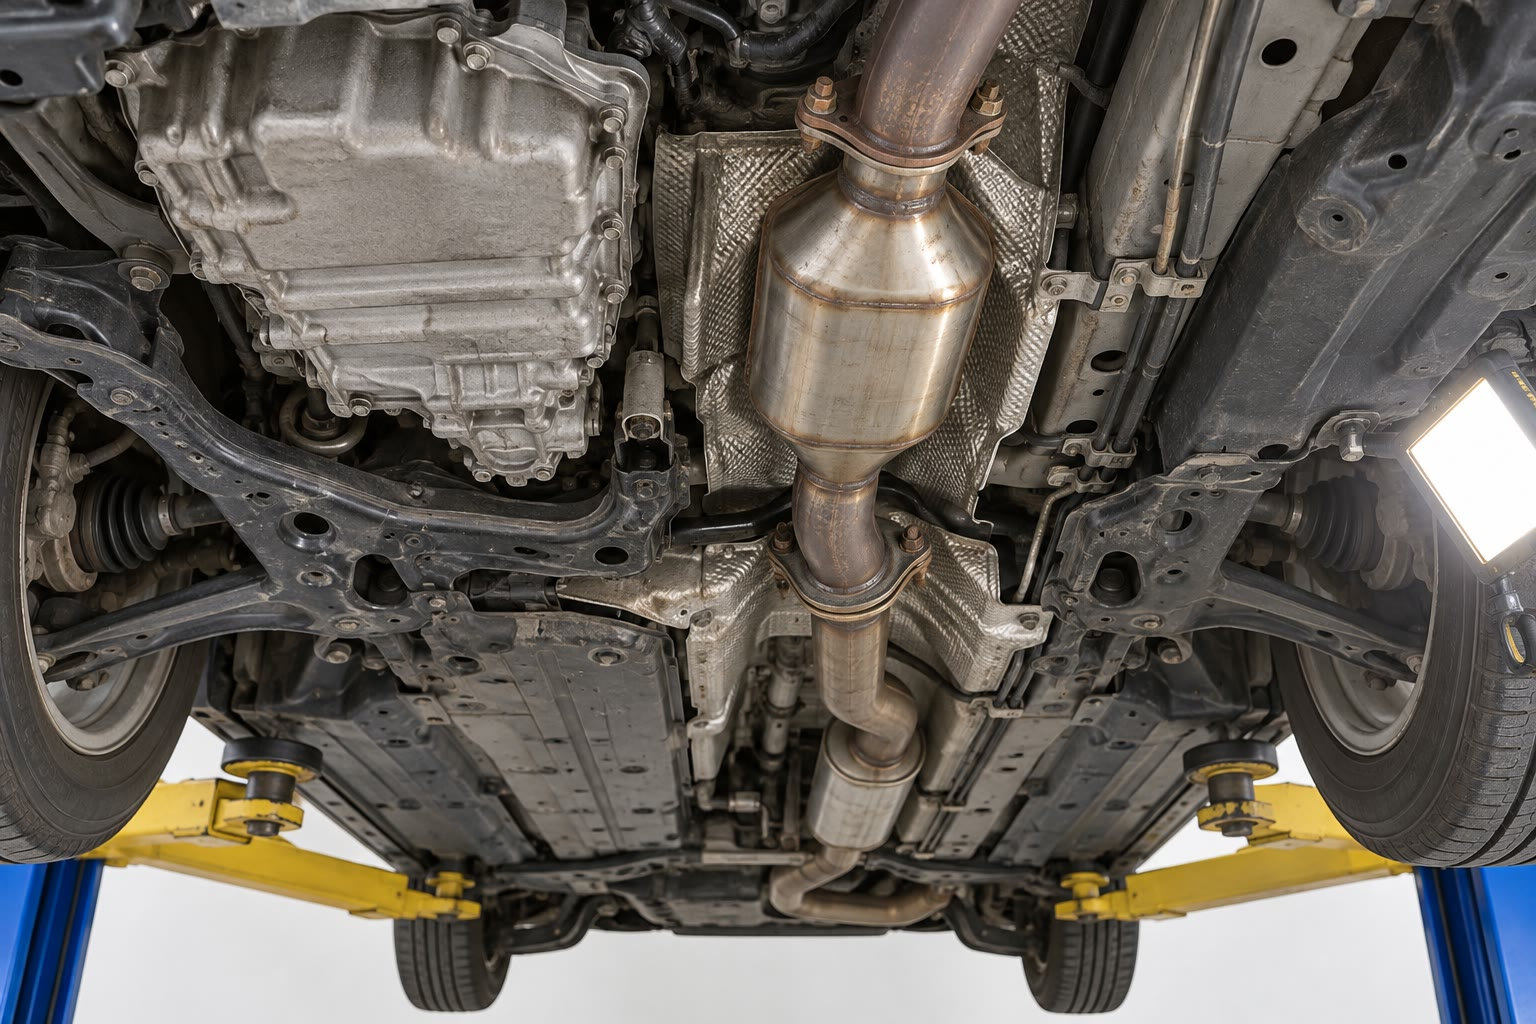
\includegraphics[width=0.5\linewidth]{images/book2/ai/b1-09-catalytic-converter.jpg}

{\small The underside of a car: the canister in the exhaust line is a
catalytic converter, a heterogeneous \omterm{def:b1:elementary-steps:catalyst}{catalyst} on whose metal surface the
exhaust gases react.}
\end{omfigure}

\begin{definition}[Kinetic and thermodynamic control]\label{def:b1:elementary-steps:control}
When a reactant can give two products by competing paths, the reaction is
under \emph{kinetic control}\index{kinetic control} if the product
proportions are fixed by the rates of formation (the product of lower
barrier dominates), and under \emph{thermodynamic
control}\index{thermodynamic control} if the paths are reversible and the
system reaches equilibrium (the more stable product dominates).
\end{definition}

\begin{example}[Choosing the product]\label{ex:b1:elementary-steps:control}
A reactant gives B over a barrier of \qty{50}{kJ/mol} ($\Delta E =
\qty{-10}{kJ/mol}$) and C over a barrier of \qty{70}{kJ/mol} ($\Delta E =
\qty{-40}{kJ/mol}$). At \qty{300}{K} and short times, with equal
\omterm{def:b1:rate-laws:activation-energy}{pre-exponential factors}, B forms $\exp(20000/(8.314 \times 300)) \approx
3000$ times faster than C: \omterm{def:b1:elementary-steps:control}{kinetic control} gives B. At high temperature
and long times, B returns over its small reverse barrier, C does not, and
the system ends as C: \omterm{def:b1:elementary-steps:control}{thermodynamic control}.
\end{example}

\begin{history}[Catalysis, 1835]
In 1835 the Swedish chemist Jöns Jacob Berzelius gathered under one word
a dozen puzzling observations --- starch turned into sugar by acids,
hydrogen peroxide decomposed by metals, alcohol oxidised on platinum ---
and called the hidden force at work ``catalytic''. It took the kinetics of
the end of the century, with Wilhelm Ostwald, to define a \omterm{def:b1:elementary-steps:catalyst}{catalyst} as a
species that changes the rate of a reaction and not its equilibrium.
\end{history}

\section{Exercises}

\begin{exercise}[$\star$]\label{exo:b1:elementary-steps:1}
Give the \omterm{def:b1:elementary-steps:elementary-step}{molecularity} of each step and say which steps can be elementary:
(a) $\ce{N2O5 -> NO2 + NO3}$; (b) $\ce{NO + NO3 -> 2NO2}$;
(c) $\ce{2H2 + O2 -> 2H2O}$; (d) $\ce{O + O2 + N2 -> O3 + N2}$.
\end{exercise}

\begin{exercise}[$\star$]\label{exo:b1:elementary-steps:2}
Write the \omterm{def:b1:rate-laws:order}{rate law} of the \omterm{def:b1:elementary-steps:elementary-step}{elementary steps} $\mathrm{A} + \mathrm{B} \to
\mathrm{C}$, $2\,\mathrm{A} \to \mathrm{B}$ and $\mathrm{A} \to \mathrm{B} +
\mathrm{C}$. Why can the \omterm{def:b1:rate-laws:order}{rate law} of an overall reaction not be written from
its equation?
\end{exercise}

\begin{exercise}[$\star$]\label{exo:b1:elementary-steps:3}
On the two-step \omterm{def:b1:elementary-steps:energy-profile}{energy profile} drawn in this chapter (intermediate at
30, \omterm{def:b1:elementary-steps:energy-profile}{transition states} at 70 and 55, products at $-40$, in
\unit{kJ/mol} above the reactants), identify the intermediate, the
\omterm{def:b1:elementary-steps:energy-profile}{transition states} and the \omterm{def:b1:elementary-steps:rds}{rate-determining step}. Is the first step endothermic or exothermic?
\end{exercise}

\begin{exercise}[$\star$]\label{exo:b1:elementary-steps:4}
A \omterm{def:b1:elementary-steps:catalyst}{catalyst} multiplies the forward \omterm{def:b1:rate-laws:order}{rate constant} of an \omterm{def:b1:elementary-steps:elementary-step}{elementary step} by
$10^4$. By how much does it multiply the reverse \omterm{def:b1:rate-laws:order}{rate constant}? the
equilibrium constant? the time needed to reach equilibrium?
\end{exercise}

\begin{exercise}[$\star\star$]\label{exo:b1:elementary-steps:5}
For $\mathrm{A} \to \mathrm{B} \to \mathrm{C}$ with $k_1 =
\qty{0.10}{s^{-1}}$ and $k_2 = \qty{0.30}{s^{-1}}$, compute $t_{\max}$ and
the largest concentration of $\mathrm{B}$, in units of $a_0$.
\end{exercise}

\begin{exercise}[$\star\star$]\label{exo:b1:elementary-steps:6}
For $\mathrm{A} \underset{k_{-1}}{\overset{k_1}{\rightleftharpoons}}
\mathrm{I} \xrightarrow{k_2} \mathrm{P}$, all steps of order 1, apply the
\omterm{def:b1:elementary-steps:qssa}{steady-state approximation} to $\mathrm{I}$ and show that $v =
\frac{k_1k_2}{k_{-1} + k_2}[\mathrm{A}]$. Discuss the cases $k_2 \gg
k_{-1}$ and $k_2 \ll k_{-1}$.
\end{exercise}

\begin{exercise}[$\star\star$]\label{exo:b1:elementary-steps:7}
Iodide ions catalyse the decomposition of hydrogen peroxide:
\ce{H2O2 + I- -> H2O + IO-} (slow), then \ce{H2O2 + IO- -> H2O + O2 + I-}
(fast). Write the overall equation, identify the \omterm{def:b1:elementary-steps:catalyst}{catalyst} and the
intermediate, and give the \omterm{def:b1:rate-laws:order}{rate law}.
\end{exercise}

\begin{exercise}[$\star\star$]\label{exo:b1:elementary-steps:8}
A step forms a carbocation from a neutral molecule, a strongly uphill
process. Using the Hammond postulate, explain why a substituent that
stabilises the carbocation also speeds the step.
\end{exercise}

\begin{exercise}[$\star\star$]\label{exo:b1:elementary-steps:9}
In \cref{ex:b1:elementary-steps:control}, compute the ratio of the \omterm{def:b1:rate-laws:order}{rate
constants} of formation of B and C at \qty{300}{K} and at \qty{600}{K}.
Comment.
\end{exercise}

\begin{exercise}[$\star\star\star$]\label{exo:b1:elementary-steps:10}
A gas $\mathrm{A}$ decomposes after being activated by collision with any
molecule $\mathrm{M}$: $\mathrm{A} + \mathrm{M} \rightleftharpoons
\mathrm{A}^* + \mathrm{M}$ ($k_1$, $k_{-1}$), then $\mathrm{A}^* \to
\mathrm{P}$ ($k_2$). With the \omterm{def:b1:elementary-steps:qssa}{steady-state approximation} for
$\mathrm{A}^*$, find $v$, and show that the reaction is of order 1 at high
pressure and of order 2 at low pressure.
\end{exercise}

\begin{exercise}[$\star\star\star$]\label{exo:b1:elementary-steps:11}
Prove the formula for $[\mathrm{B}](t)$ of
\cref{thm:b1:elementary-steps:consecutive} and treat the special case
$k_1 = k_2 = k$, for which $[\mathrm{B}] = a_0kt\,\eu^{-kt}$.
\end{exercise}

\begin{exercise}[$\star\star\star$]\label{exo:b1:elementary-steps:12}
The overall reaction $\mathrm{A} + 2\,\mathrm{B} \to \mathrm{P} +
\mathrm{C}$ has the experimental \omterm{def:b1:rate-laws:order}{rate law} $v =
k[\mathrm{A}][\mathrm{B}]^2/[\mathrm{C}]$. Propose a mechanism with a fast
pre-equilibrium that explains it.
\end{exercise}

\section{Problem: Why Nitrogen Monoxide Oxidises Faster in the Cold}

\begin{problem}[{Weekend problem --- the third-order oxidation of nitrogen
monoxide, a pre-equilibrium through the dimer \ce{N2O2}, the steady-state
treatment, and a negative apparent \omterm{def:b1:rate-laws:activation-energy}{activation energy}}]
\label{pb:b1:elementary-steps:1}
For \ce{2NO(g) + O2(g) -> 2NO2(g)}, initial-rate measurements at
\qty{300}{K} give (rates in \unit{mol.L^{-1}.s^{-1}}):
\begin{center}
\begin{tabular}{cccc}
\hline
experiment & $[\ce{NO}]_0$ (mol/L) & $[\ce{O2}]_0$ (mol/L) & $v_0$ \\
\hline
1 & \num{1.0e-3} & \num{1.0e-3} & \num{1.0e-5} \\
2 & \num{2.0e-3} & \num{1.0e-3} & \num{4.0e-5} \\
3 & \num{1.0e-3} & \num{2.0e-3} & \num{2.0e-5} \\
\hline
\end{tabular}
\end{center}
The \omterm{def:b1:rate-laws:order}{rate constant} found at \qty{400}{K} is ten times smaller than at
\qty{300}{K}. Take $R = \qty{8.314}{J/(mol.K)}$.
The proposed mechanism is
\[
  \ce{2NO <=> N2O2} \ \ (k_1, k_{-1}, \text{fast}), \qquad
  \ce{N2O2 + O2 -> 2NO2} \ \ (k_2, \text{slow}).
\]

\medskip
\noindent\textbf{Part I --- The observed law.}
\begin{enumerate}
  \item Find the \omterm{def:b1:rate-laws:order}{partial orders} with respect to \ce{NO} and \ce{O2}.
  \item Write the \omterm{def:b1:rate-laws:order}{rate law} and compute $k$ at \qty{300}{K}, with its unit.
  \item Could the reaction be a single termolecular step? Give an argument.
  \item Compute the apparent \omterm{def:b1:rate-laws:activation-energy}{activation energy} from the two temperatures.
  \item Why is a negative \omterm{def:b1:rate-laws:activation-energy}{activation energy} impossible for an \omterm{def:b1:elementary-steps:elementary-step}{elementary
        step}?
  \item Write the rates of disappearance of \ce{NO} and \ce{O2} in terms of
        $v$.
\end{enumerate}

\medskip
\noindent\textbf{Part II --- The pre-equilibrium.}
\begin{enumerate}[resume]
  \item Check that the two steps add up to the overall reaction. Name the
        intermediate.
  \item Give the \omterm{def:b1:elementary-steps:elementary-step}{molecularity} of each step.
  \item Write the rate of the slow step.
  \item Express $[\ce{N2O2}]$ with the \omterm{def:b1:elementary-steps:pre-equilibrium}{pre-equilibrium approximation}.
  \item Deduce the \omterm{def:b1:rate-laws:order}{rate law} and compare with experiment.
  \item Express the observed constant with $k_1$, $k_{-1}$ and $k_2$.
\end{enumerate}

\medskip
\noindent\textbf{Part III --- The steady state.}
\begin{enumerate}[resume]
  \item Write $\dd[\ce{N2O2}]/\dd t$ for the full mechanism.
  \item Apply the \omterm{def:b1:elementary-steps:qssa}{steady-state approximation} and express $[\ce{N2O2}]$.
  \item Deduce the \omterm{def:b1:rate-laws:order}{rate law} $v = \dfrac{k_1k_2[\ce{NO}]^2[\ce{O2}]}{k_{-1} +
        k_2[\ce{O2}]}$.
  \item In which limit does it reduce to the result of Part II?
  \item What would the orders become in the opposite limit?
  \item Which limit do the measurements of Part I support?
\end{enumerate}

\medskip
\noindent\textbf{Part IV --- The apparent \omterm{def:b1:rate-laws:activation-energy}{activation energy}.}
Each step follows the \omterm{thm:b1:rate-laws:arrhenius}{Arrhenius law}, with activation energies $E_1 =
\qty{2}{kJ/mol}$, $E_{-1} = \qty{40}{kJ/mol}$ and $E_2 =
\qty{15}{kJ/mol}$.
\begin{enumerate}[resume]
  \item Write $\ln k$ in terms of the logarithms of $k_1$, $k_{-1}$ and
        $k_2$.
  \item Deduce $E_a = E_1 - E_{-1} + E_2$.
  \item Interpret: why can a combination of \omterm{def:b1:elementary-steps:elementary-step}{elementary steps} have a
        negative apparent \omterm{def:b1:rate-laws:activation-energy}{activation energy}?
  \item Sketch the \omterm{def:b1:elementary-steps:energy-profile}{energy profile}: where is the second \omterm{def:b1:elementary-steps:energy-profile}{transition state},
        relative to the reactants \ce{2NO + O2}?
  \item By what factor would the rate change between 300 and \qty{400}{K}
        with this value?
  \item Compute the apparent \omterm{def:b1:rate-laws:activation-energy}{activation energy} from the step values, and
        compare with Part I.
\end{enumerate}
\end{problem}
